\clearpage
\makeatletter
\efloat@restorefloats
\makeatother


\begin{appendix}
\hypertarget{supplementary-analysis}{%
\section{Supplementary Analysis}\label{supplementary-analysis}}

Additional analyses were conducted to clarify the effect of task on
classification accuracy. These supplementary analyses were not seen as
central to the current study, but could prove to be informative to
researchers attempting to replicate or extend these findings in the
future. The results from the primary analyses showed that classification
accuracies were the lowest for the Memorize condition, but these
findings did not indicate if the Memorize condition was adding noise to
the data, or was providing redundant information to the model. To
further understand why classification accuracy was lower for the
Memorize condition than it was for the Search or Rate condition, the
Exploratory and Confirmatory timeline datasets were systematically
batched into subsets with the Search (S), Memorize (M), or Rate (R)
condition removed (i.e., \(\varnothing\)MR, S\(\varnothing\)R,
SM\(\varnothing\)).

All of the data subsets analyzed in this supplementary analysis were
decoded with better than chance accuracy (see Figure
@ref(fig:supp-chance)). The same pattern of results was observed in both
the Exploratory and Confirmatory datasets. When the Memorize condition
was removed, classification accuracy improved (see Table
@ref(tab:supp-comparisons)). When the Rate condition was removed,
classification was the worst. When the Memorize condition was included,
the Memorize condition was more accurately predicted than the Search and
Rate conditions (see Figure @ref(fig:supp-conf-matrices)).

\begin{figure}
\centering
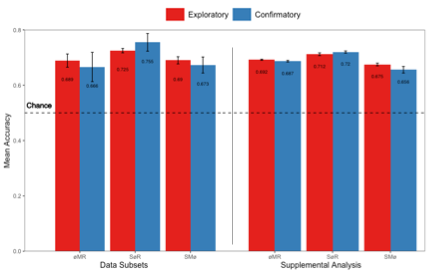
\includegraphics{supplementary_analysis/recalc_orig_accs/recalc_bar_graph.png}
\caption{(\#fig:supp-chance)The graph represents the average accuracy
reported for each subset of the Exploratory and Confirmatory timeline
data for the supplementary analysis and the re-calculated accuracies
from the primary analyses. All of the data subsets were decoded at
levels better than chance (50\%). The error bars represent standard
errors.}
\end{figure}

\begin{table}[!h]
    \centering
    \caption{Supplementary Subset Comparisons}
    \label{tab:supp-comparisons}
    \begin{tabular}{l c c c c}
         & \multicolumn{2}{c}{Exploratory} & \multicolumn{2}{c}{Confirmatory} \\
        \hline
        Comparison & \textit{t} & \multicolumn{1}{c|}{\textit{p}} & \textit{t} & \textit{p} \\
        \hline
        $\varnothing$MR vs. S$\varnothing$R & 3.248 & \multicolumn{1}{c|}{.008} & 3.094 & .012 \\
        $\varnothing$MR vs. SM$\varnothing$ & 2.875 & \multicolumn{1}{c|}{.021} & 2.923 & .018 \\
        S$\varnothing$R vs. SM$\varnothing$ & 6.123 & \multicolumn{1}{c|}{< .001} & 6.017 & < .001 \\
        \hline
    \end{tabular}
\end{table}

\begin{figure}
\centering
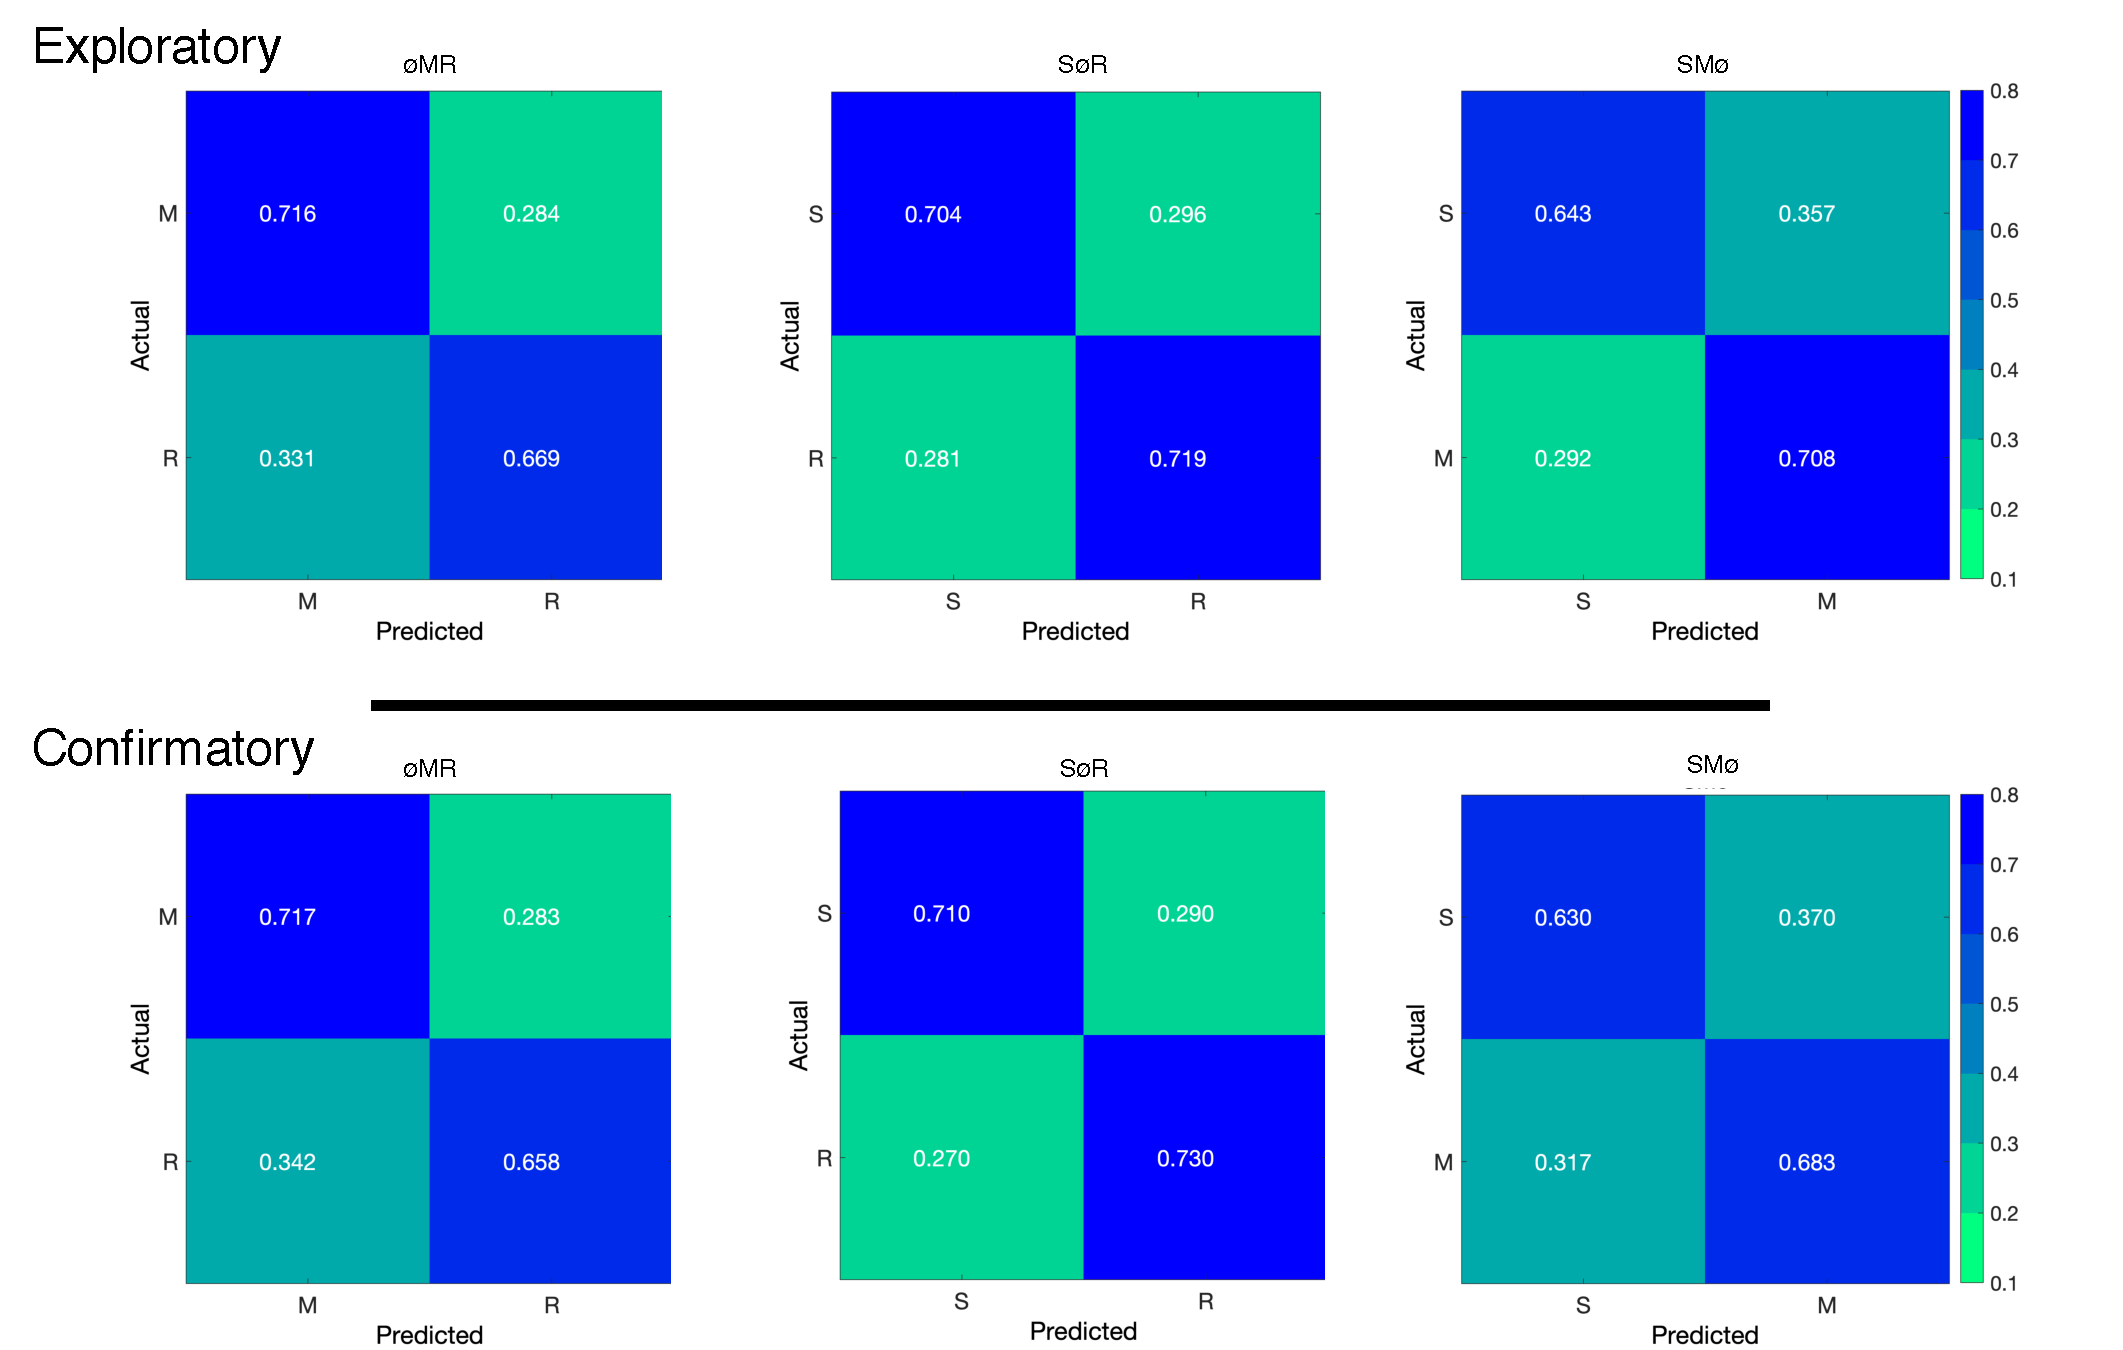
\includegraphics{supplementary_analysis/confusion_matrices/supp_conf_matrices.pdf}
\caption{(\#fig:supp-conf-matrices)The confusion matrices represent the
average classification accuracies for each condition of the timeline
data (S = Search, M = Memorize, R = Rate). The vertical axis of the
confusion matrices represents the actual condition for trial. The
horizontle axis of the confusion matrices represents the condition that
was predicted by the model.}
\end{figure}

Overall, the accuracies for all of the data subsets observed in the
supplementary analysis were higher than the accuracies observed in the
main analysis. Chance accuracy levels for the primary analysis was 33\%,
but because one of the tasks was removed from each element observed in
the supplementary analyses, chance accuracy for these analyses was 50\%.
Given the data analyzed for these supplementary purposes have different
thresholds of chance performance, any conclusions drawn from a
comparison between the primary and supplementary datasets could be
misleading. For this reason, we revisited the results from the primary
analyses and re-calculated the accuracies to be equivalent to a 50\%
chance threshold. The accuracies were recalculated using the following
formula: Accuracy\(_{New}\) = Accuracy\(_{Original}\) /
(Hits\(_{Original}\) + Misses\(_{Original}\)). For example, accuracy for
the Search classification for S\(\varnothing\)R would be calculated with
the following: Search\(_{Hits}\) = Hits\(_{Search}\) /
(Hits\(_{Search}\) + Misses\(_{Search}\)), where Misses\(_{Search}\) is
the ratio of Search trials that were misclassified as Rate.

The re-calculated confusion matrices for each category are presented in
Figure @ref(fig:recalc-conf-matrices). The general pattern of findings
presented in the re-calculated confusion matrices was the same as the
pattern that can be seen in the supplementary analysis. This is also
true for the pattern of results for the overall accuracies (see Figure
@ref(fig:supp-chance)). In both analyses, the subsets that include the
Memorize trials were classified with lower accuracy than the other data
subsets. Furthermore, a closer look at the confusion matrices shows that
the Memorize conditions were most often confused with the other two
conditions. Because the Memorize condition was mis-classified to a
similar extent when paired with Search or Rate conditions, and these
mis-classifications affected the overall accuracies to a similar extent,
we believe it is likely that there was an increased presence of noise in
the eye movement data for the Memorize trials.

\begin{figure}
\centering
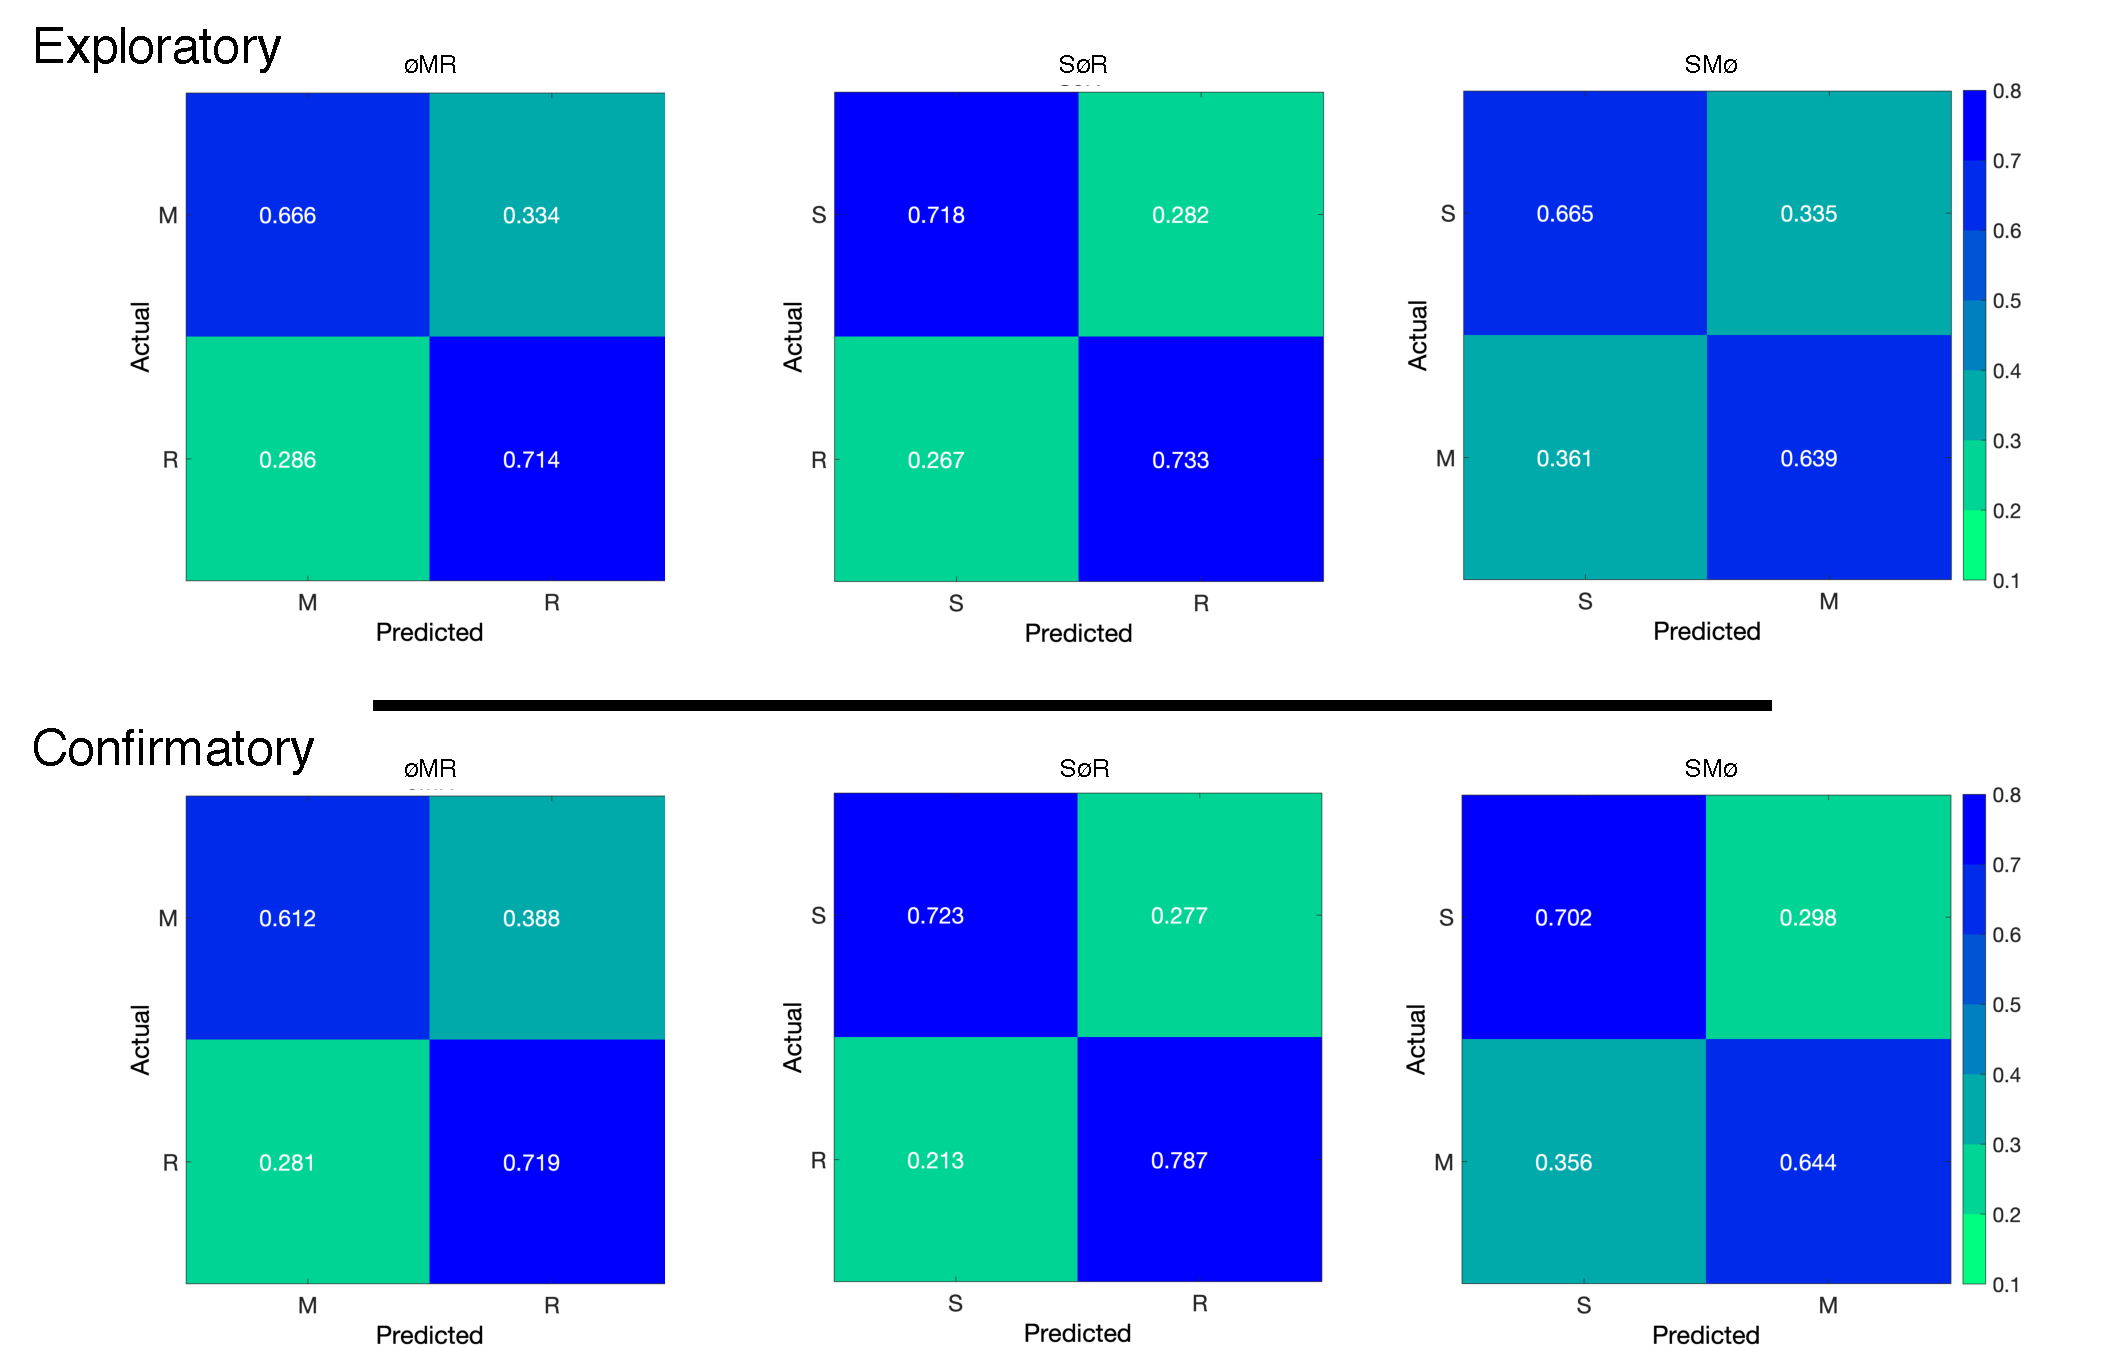
\includegraphics{supplementary_analysis/recalc_orig_accs/confusion_matrices/recalc_conf_matrices.pdf}
\caption{(\#fig:recalc-conf-matrices)The confusion matrices represent a
re-calculation of the classification accuracies for each category from
the primary analysis. This re-calculation is meant to make the
accuracies presented in the primary analysis (chance = 33\%) equivalent
to the classification accuracies presented in the supplementary analysis
(chance = 50\%).}
\end{figure}
\end{appendix}
